\documentclass{beamer}

\usepackage{listings} \lstset{numbers=left, numberstyle=\tiny, numbersep=5pt} \lstset{language=C}
\usepackage{wrapfig}
\usepackage{beamerbaseverbatim}
%\usepackage{ngerman}
\usepackage{beamerthemesplit}
\usepackage[latin1]{inputenc}
\usepackage[T1]{fontenc}

\title{Einf\"uhrung in die Microcontroller Programmierung}
\author{S\"oren Heisrath}
\date{30.10.2009}

\begin{document}

\frame{\titlepage}

\section[Grundfunktionen des Microcontrollers]{}
% \frame{\tableofcontents}

% =========================== PINS & PORTS ===========================
\subsection{Pins \& Ports}
\frame
{
	\frametitle{Pins \& Ports}
	Funktionen der Pins
	\begin{itemize}
		\item Einfache Ein/Ausgabe (An/Aus)
		\item Spannungsmessung / ADC (Sp\"ater)
		\item Automatische PWM mit Timern
		\item Interrupts
		\item UART (Serielle Schnittstelle)
		\item ...
	\end{itemize}

}
\frame
{
	\frametitle{Beispiel: Atmega32}
	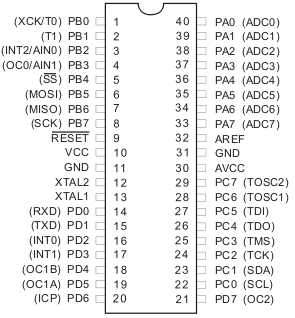
\includegraphics[scale=0.6]{img/ioports}
}

\frame
{
	\frametitle{Ports}
	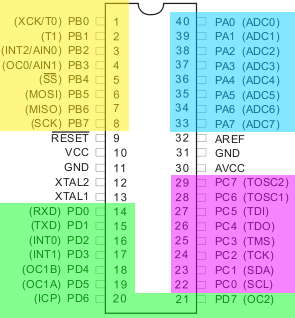
\includegraphics[scale=0.6]{img/ioports_hl}
}

\subsection{Interrupts}
\frame
{
	\frametitle{Interrupts}
	\begin{centering}
		\large{Interrupts sind Unterbrechungen des Hauptprogramms.}
	\end{centering}
}
\frame
{
	\frametitle{Aufruf eines Interrupts}
	\begin{enumerate}
		\item Gerade laufendes Programm wird angehalten
		\item Interrupt Routine wird ausgef\"uhrt
		\item Hauptporgramm wird fortgesetzt
	\end{enumerate}
	\large{Stichwort: Interrupt Vektor}
}
\frame
{
	\frametitle{Verschiedene Arten von Interrupts}
	Beispiele:
	\begin{itemize}
		\item Pegel\"anderung an einem Pin
		\item Timer\"uberlauf
		\item Timer Compare Match
		\item ADC Interrupt
		\item ...
	\end{itemize}
}
\subsection{Timer/Counter}
\frame
{
	\frametitle{Anwendung}
	\begin{itemize}
		\item Z\"ahler
		\item PWM generator
		\item Periodische Ausf\"uhrung von Code
	\end{itemize}
}
\frame
{
	\frametitle{Funktionen}
	\begin{itemize}
		\item Fest eingestellter Takt (z.B. 1/64 des Taktes)
		\item 8 oder 16 Bit-Z\"ahler
		\item 2 verschiedene Interrupts: Overflow \& Compare Match
		\item Automatische Ausgabe (PWM)
	\end{itemize}
}
\section{Das erste Programm}
\subsection{Datenrichtungen}
\frame
{
	\frametitle{Das Data Direction Register}
	Das DDR besteht aus 8 Bits, die die Datenrichtung vorgeben
	\begin{itemize}
		\item 1 = Ausgang
		\item 0 = Eingang
	\end{itemize}
}
\frame
{
	\frametitle{Beispiel}
	Schalte Pin 0 und 1 als Ausgang, den Rest auf Eingang:
	\par
	\lstinline|DDRB = \_BV(PB0) \| \_BV(PB1);|
}
\subsection{Logische Operationen}
\frame
{
	\frametitle{ODER Verkn\"upfung}
	Setzt alle Bits auf 1, die in den Operanden auf 1 sind.\\
	Symbol: |\\
	Beispiel:
	\par\lstinline|variable = 0x40 \| 0x02; /* ergebnis: 0x42 */|
}
\frame
{
	\frametitle{UND Verkn\"upfung}
	Setzt alle Bits auf 1, die bei beiden Operanden an gleicher Stelle auf 1 gesetzt sind.\\
	Symbol: \&\\
	Beispiel:
	\par\lstinline|variable = 0x42 \& 0x02; /* ergebnis: 0x02 */|
}
\frame
{
	\frametitle{Negation}
	Kippt alle Bits um
	Symbol: ~
	Beispiel:
	\par\lstinline|variable = ~0x04; /* ergebnis: 0xFB */|
}
\subsection{Das erste Programm}
\frame
{
	\begin{small}
	\lstinputlisting[frame=single]{1st.c}
	\end{small}
}
\subsection{Eingangswerte lesen}
\frame
{
	\begin{small}
	\lstinputlisting[frame=single]{input.c}
	\end{small}
}
\subsection{Definierte Werte}
\frame
{
	Pullup Widerst\"ande geben Eing\"angen definierte Werte:
	\begin{small}
	\lstinputlisting[frame=single]{pullup.c}
	\end{small}
	Die Reihenfolge ist wichtig beim Anschalten der Pullups: Die bin\"are 1
	sollte erst NACH setzen des DDRs auf Eingang gesetzt werden.
}
\subsection{Entprellen}
\frame
{
	Entprellen:
	\begin{small}
	\lstinputlisting[frame=single]{prell.c}
	Hier wird abgefragt, ob der button NICHT gedr\"uckt ist.
	Um abzufragen, ob der Button am Pullup gedr\"uckt ist, schreibt man:
	\lstinline|... if (!(PINA & (_BV(PA0)))) ...|
	\end{small}
}


\section{Timer/Counter nutzen}
\frame
{
	Vorgehen:
	\begin{enumerate}
		\item Datenblatt konsultieren
		\item Geeigneten Timer f\"ur Anwendung aussuchen
		\item Register raussuchen:
		\begin{itemize}
			\item Prescaler
			\item Timer Control register
			\item ggf. Interrupts
		\end{itemize}
	\end{enumerate}
}
\frame
{
	Initialisierung:
	\begin{small}
	\lstinputlisting[frame=single]{timer_init.c}
	\end{small}
}
\frame
{
	Timer ISR:
	\begin{small}
	\lstinputlisting[frame=single]{timer_isr.c}
	\end{small}
}
\section{Und jetzt..? Ein Ausblick}
\frame
{
	\frametitle{USB am AVR}
	\begin{centering}
		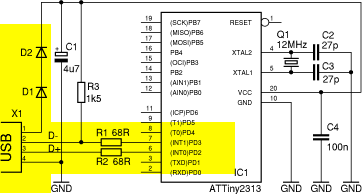
\includegraphics[scale=0.6]{img/v-usb}
		\\\url{http://www.obdev.at/vusb}
	\end{centering}
}
\frame
{
	\frametitle{Datenfunk mit RFM12}
	\begin{centering}
		\url{http://www.das-labor.org/wiki/Datenfunk_mit_dem_AVR}\\
		\url{http://www.das-labor.org/svn/trac/browser/src-atmel/microcontroller/lib/rfm12}
	\end{centering}
}
\frame
{
	\frametitle{Peripherie anschliessen}
	\begin{itemize}
		\item Display (z.B. mit HD44780 Controller)
		\item CAN Bus
		\item Serielle Schnittstelle
	\end{itemize}
}
\frame
{
	\frametitle{Weiterf\"uhrende Links}
	\url{http://www.mikrocontroller.net} - AVR GCC Tutorial
	\url{http://www.das-labor.org/wiki/Laborboard} - Projekte
}

\end{document}


